\newpage
\subsection{The role of topography}

\textbf{i)} Choosing $kR_d=1.73$ and introducing topography as $H(y)=\alpha y + H_0$ gives the result seen in \autoref{fig:hovmöller_topo}. For the case when $\alpha=0$ one can see an East-moving wave-packet and Westward phase, as expected from the theory. When $\alpha$ was increased to \SI{2.29e-4}{\per\meter} and \SI{4.58e-4}{\per\meter} one can observe less propagation on the same timespan, still with Westward phase and Eastward group velocity. However, when the topography tilts in the opposing way, $\alpha=\SI{-2.29e-4}{\per\meter}$, we see an even faster moving wave compared to when there was no topography. This makes sense, since a negative tilt would only increase the "observed beta-effect". When $\alpha=\SI{8e-4}{\per\meter}$ nothing moves, as expected from the theory. More interestingly, one can observe a Westward group velocity and Eastward phase when the $\alpha$-value was set to be above the cancelling $\alpha$-value.

The parameter of $kR_d=1.73$ was chosen since this provided the faster moving group-velocity, which is good for visualization. The different alphas were chosen to reflect the role of the topography. They were chosen based on the ratio between the tilted plane at the end of the domain and the mean depth, labelled as $r$. The $\alpha$-points which were used can be seen in \autoref{tab:alpha_effects}.
\begin{table}[H]
\centering
\begin{tabular}{c c c c}
\hline
Depth ratio $r$ [-] & $\alpha\,[\mathrm{m^{-1}}]$ & Observed beta-effect & Group direction \\
\hline
$-0.2$ & $-2.29\times10^{-4}$ & enhanced $\beta_\text{eff}$ & stronger Eastward \\
$0.0$ & $0$ & normal $\beta$ & Eastward \\
$0.2$ & $2.29\times10^{-4}$ & reduced $\beta_\text{eff}$ & weak Eastward \\
$0.4$ & $4.58\times10^{-4}$ & strongly reduced $\beta_\text{eff}$ & even weaker Eastward \\
$0.7$ & $8.0\times10^{-4}$ & $\beta_\text{eff}=0$ & zero \\
$0.8$ & $9.16\times10^{-4}$ & reversed $\beta_\text{eff}$ & Westward \\
\hline
\end{tabular}
\caption{Effect of varying topographic slope $\alpha$ on Rossby wave propagation for $kR_d=1.73$. }
\label{tab:alpha_effects}
\end{table}

\begin{figure}[H]
    \centering    
    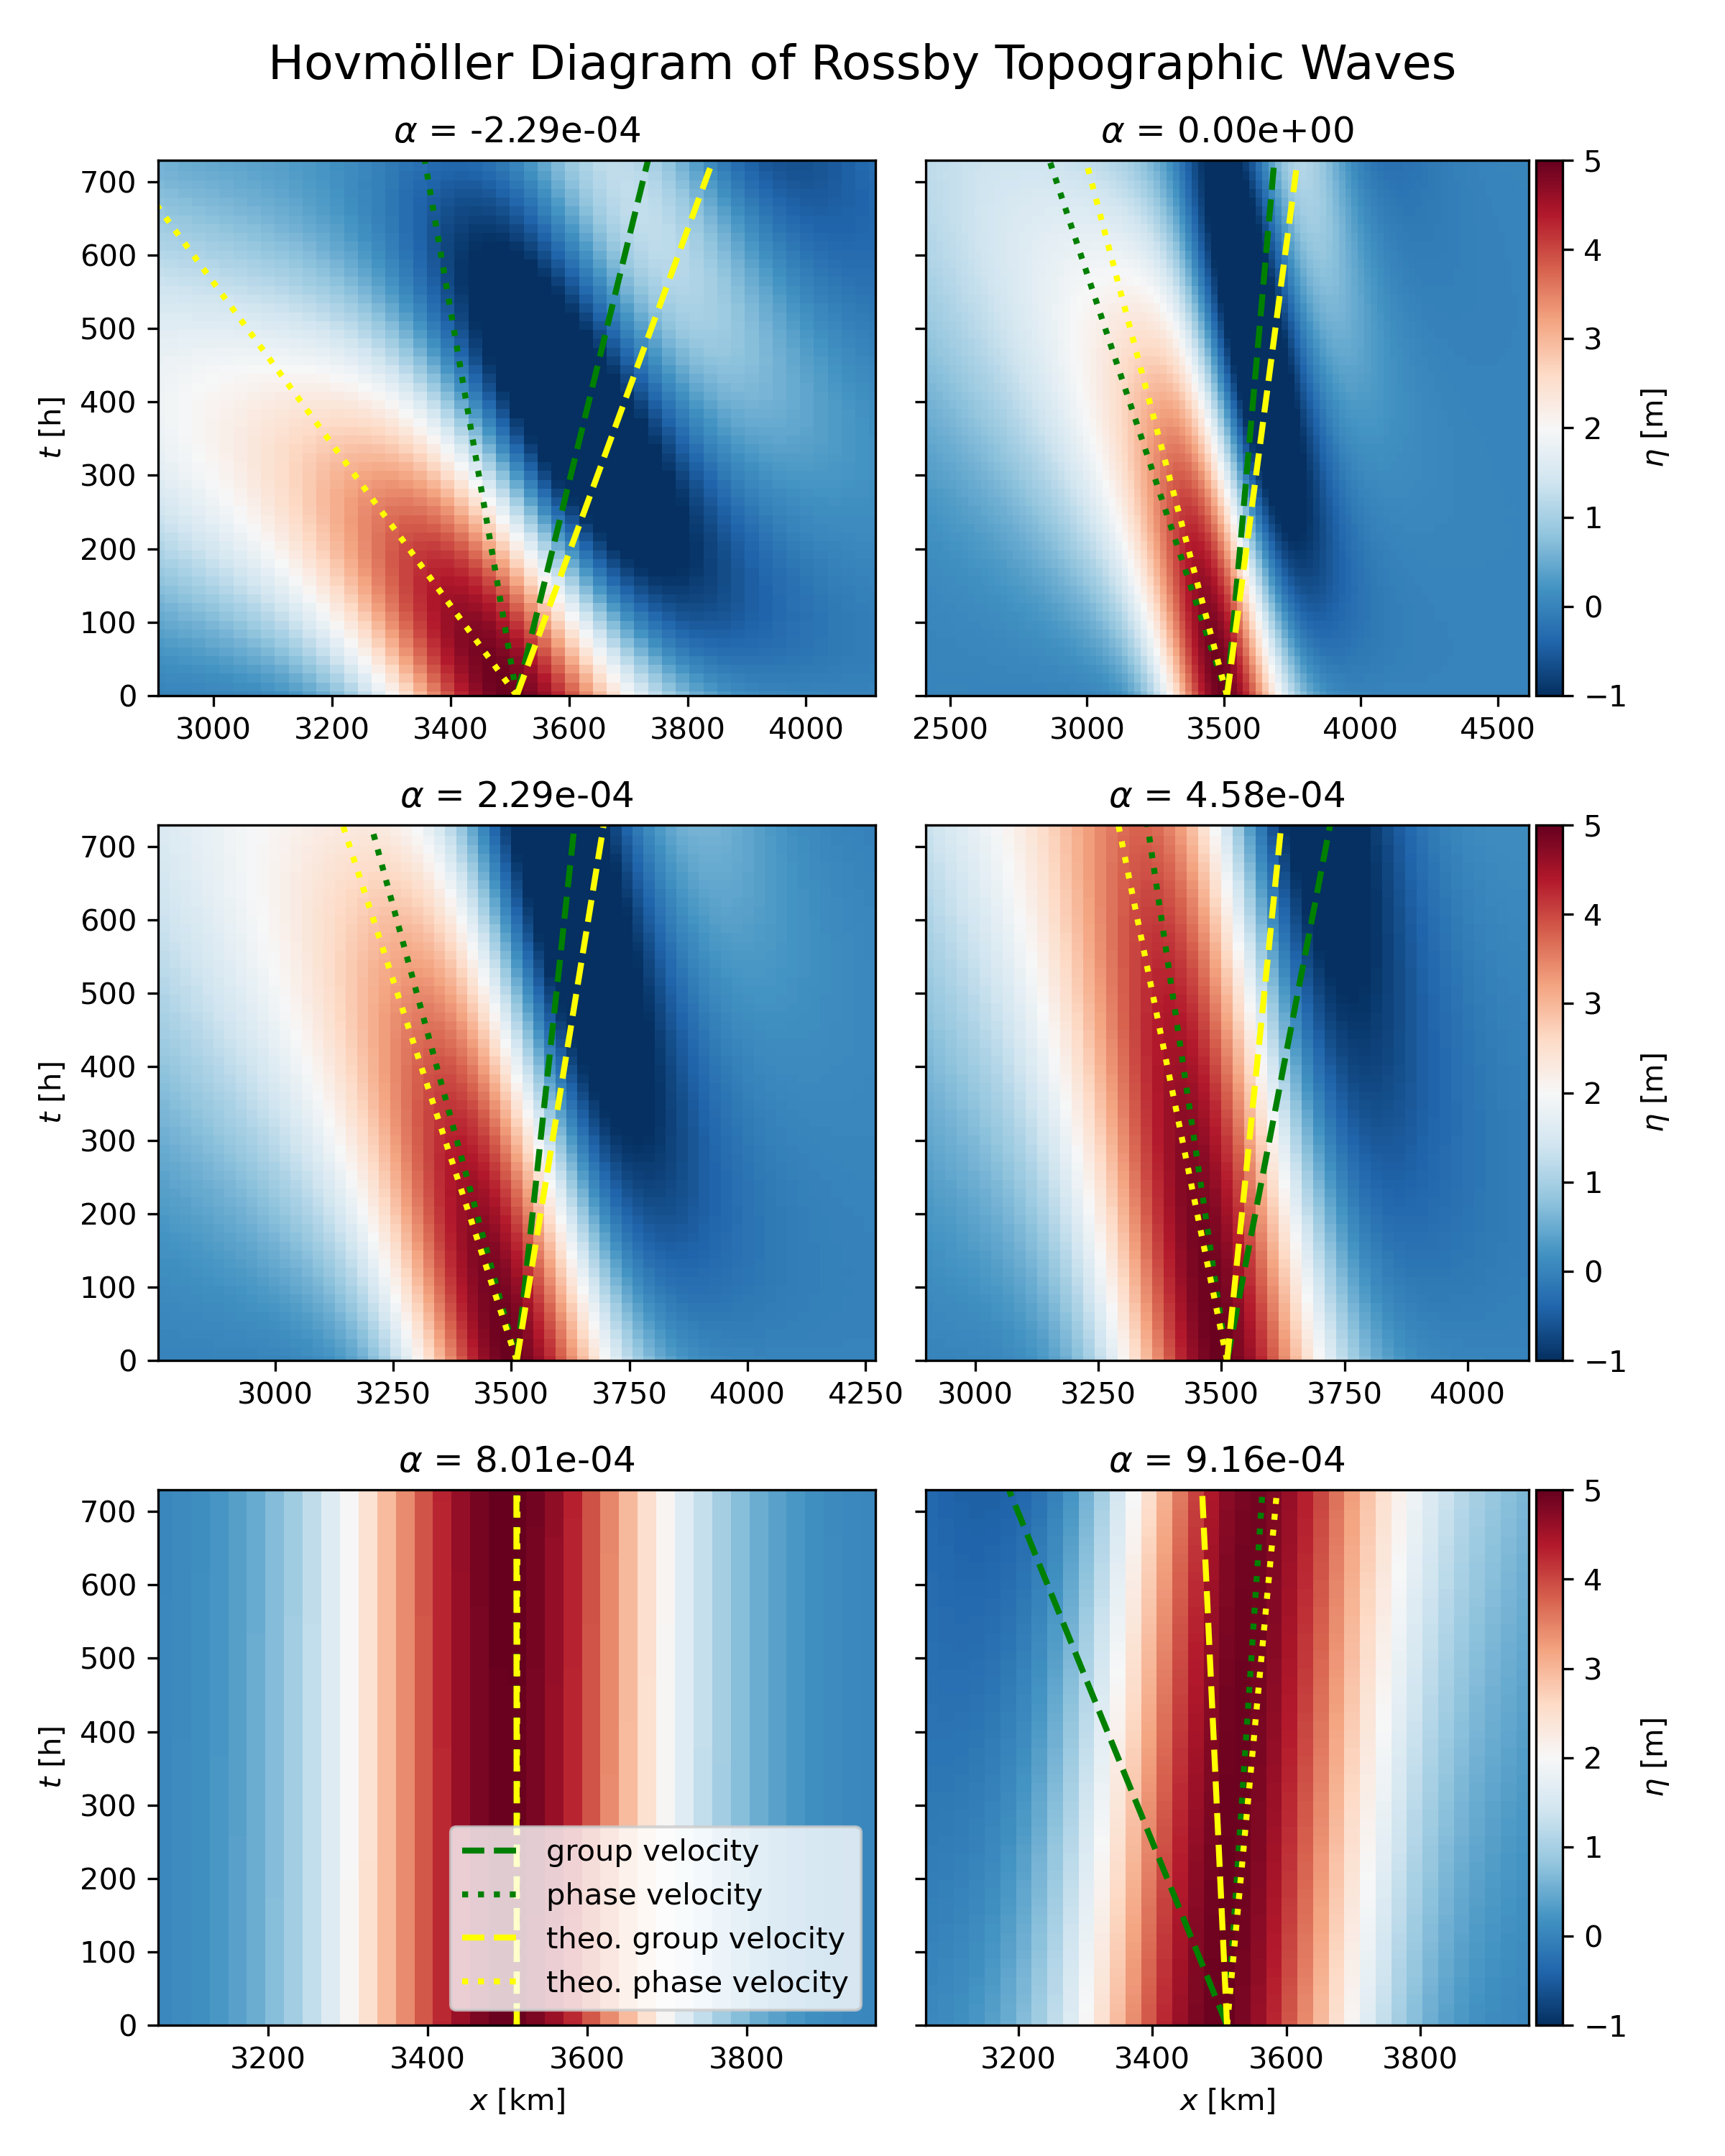
\includegraphics[width=0.6\textwidth]{Figures/hovmöller_topo.png}
    \caption{This figure shows the topographic Rossby waves for $kR_d=1.73$ as Hovmöller diagrams.}
    \label{fig:hovmöller_topo}
\end{figure}

\textbf{ii)} The same result observed in \autoref{fig:hovmöller_topo} can be seen for the entire domain in \autoref{fig:topography_contours}. There one can see results for the initial condition, 10 days, 20 days, and 30 days. An interesting observation is that even though setting $\alpha=\SI{8e-4}{\per\meter}$, the edges of the initial perturbation can still be seen to move due to the beta-effect.

\begin{figure}[H]
    \centering    
    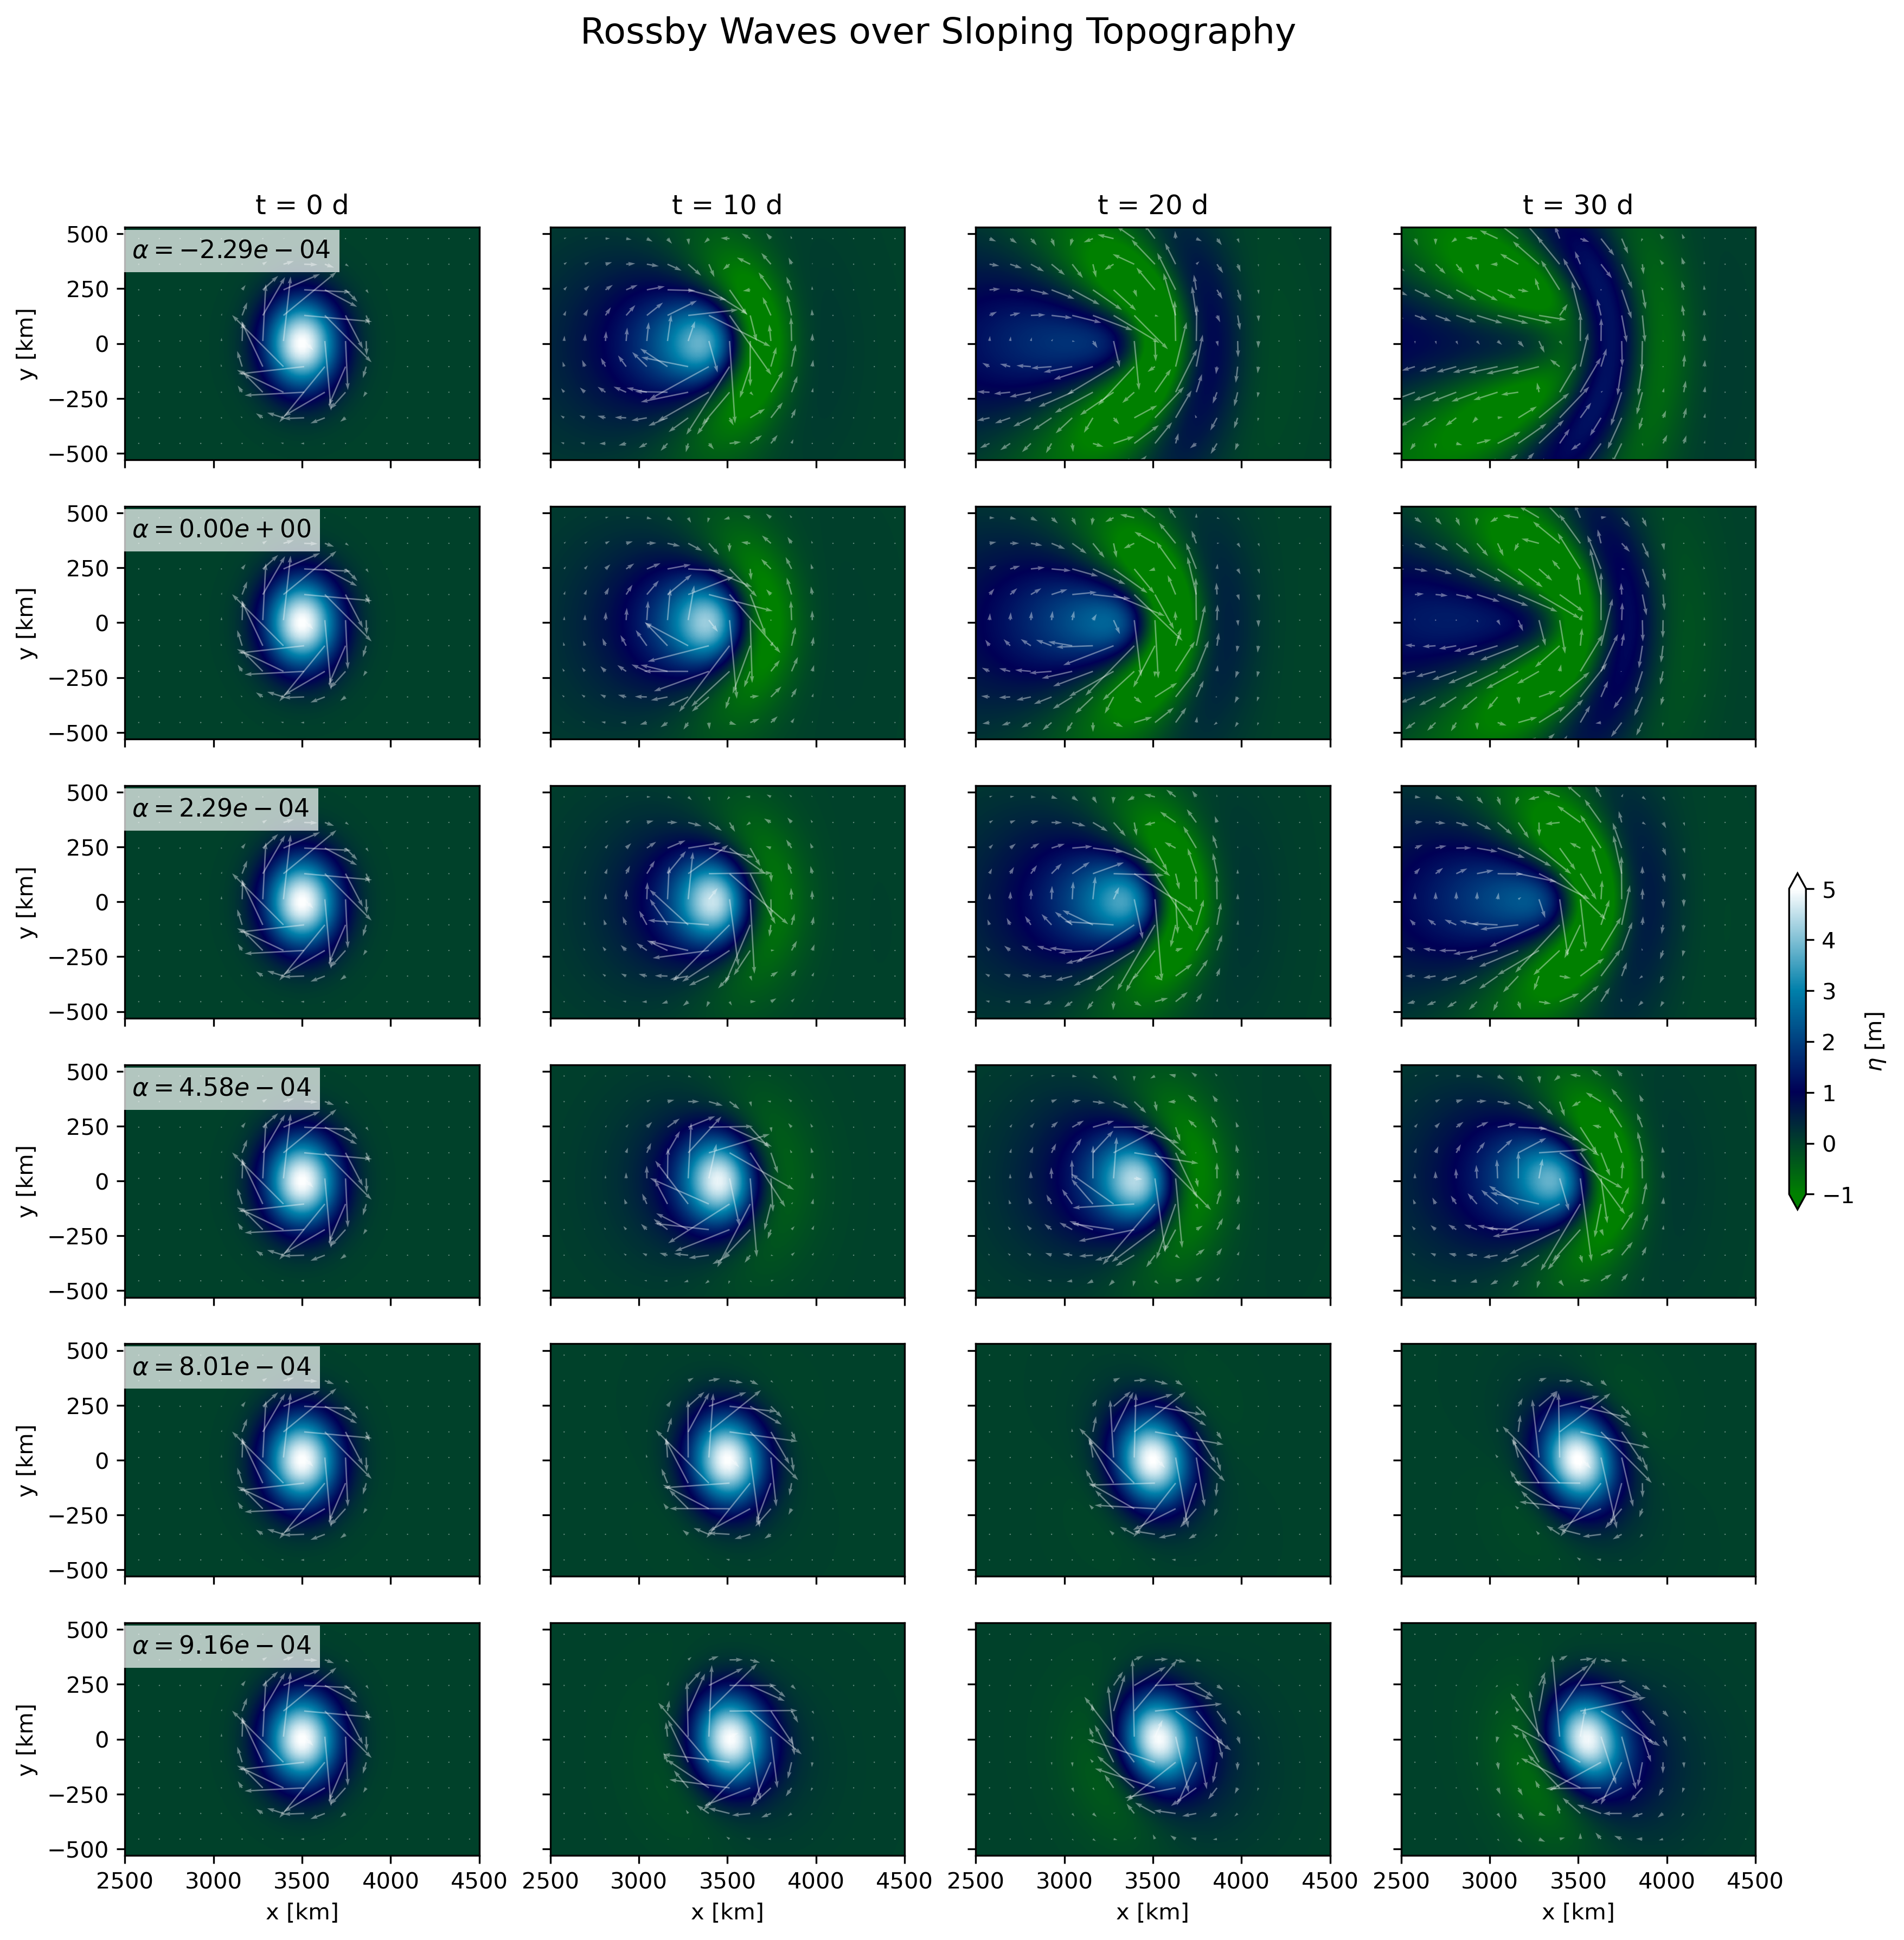
\includegraphics[width=\textwidth]{Figures/topography_contours.png}
    \caption{This figure shows the contour plots of the Rossby waves in the $xy$-plane.}
    \label{fig:topography_contours}
\end{figure}

\newpage
\textbf{iii)} In \autoref{fig:dispersion_topo} one can observe the phase and group speeds like in question 2.1 iv. Here one can see that a negative $\alpha$-value made stronger velocities, with a similar accuracy to the non-topographic curve. The middle plot with $\alpha=\SI{4.58e-4}{\per\meter}$ showed damped speeds compared to the non-topographic curve, again with similar accuracy. The $\alpha$-value with a higher value than the cancelling $\alpha$-value showed opposing speeds compared to the others. This is because the topography is now stronger than the beta-effect, which makes the Rossby wave propagate in the opposing direction. The accuracy here is still good.

\begin{figure}[H]
    \centering    
    
\includegraphics[width=\textwidth]{Figures/dispersion_topo.png}
    \caption{This figure showcases the phase and group velocities for a few different $\alpha$-values, compared to $\alpha=0$. The non-topographic $\alpha=0$ line is the orange one in all subfigures.}
    \label{fig:dispersion_topo}
\end{figure}